\chapter{Introduction}
\label{ch:introduction}

\section{Motivation}

A youth or amateur coach who wants to know how compact the team stayed in the second half, or which shape the opponent defended in, has two options today. One is to buy data: top clubs get tracking data from multi-camera systems in the stadium, from GPS vests, or from providers whose operators annotate every match by hand. The other is to watch the video again with a notepad. The first is out of reach below professional level, and the second takes hours and produces no numbers.

What these coaches usually do have is video. The question I started from was therefore a practical one: how much of the professional tactical picture (positions in metres, team shape, formations, running distances) can be recovered automatically from a single broadcast camera, and how can it be shown so that a coach actually uses it?

Off-the-shelf tools did not answer this. Commercial platforms sell their data per match and do not analyse the user's own footage. The open-source football examples, such as the Roboflow \emph{sports} repository~\cite{roboflowsports}, are notebooks that draw boxes on a clip; they do not run as a service, do not survive a crash halfway through a 45-minute video, and have no interface for a coach. I wanted a system that a non-technical user could open in a browser, upload a match to, and come back to later.

The computer vision part has become feasible: YOLOv8~\cite{yolov8} detects players and the ball, ByteTrack~\cite{bytetrack} follows them over time, and projective geometry~\cite{hartley} maps the image onto a flat pitch. The engineering part was at least as demanding. On my laptop a 30-second clip took about 25 minutes to analyse, so the analysis could never run inside a web request, and the results are only useful when they are drawn on the video they came from, frame by frame, while the camera pans.

\section{Objectives and overview}

The aim was to build \textbf{Tactical Eye}, a web platform that turns football video into tactical information without manual annotation. A user uploads a match, follows the analysis live, and then watches the video with every player marked by their position, movement paths, team shapes and heatmaps drawn on the pitch, next to a 2D tactical board, the formations of both teams, statistics and an AI-written coaching report (\autoref{fig:intro-analysis}).

\begin{figure}[htbp]
	\centering
	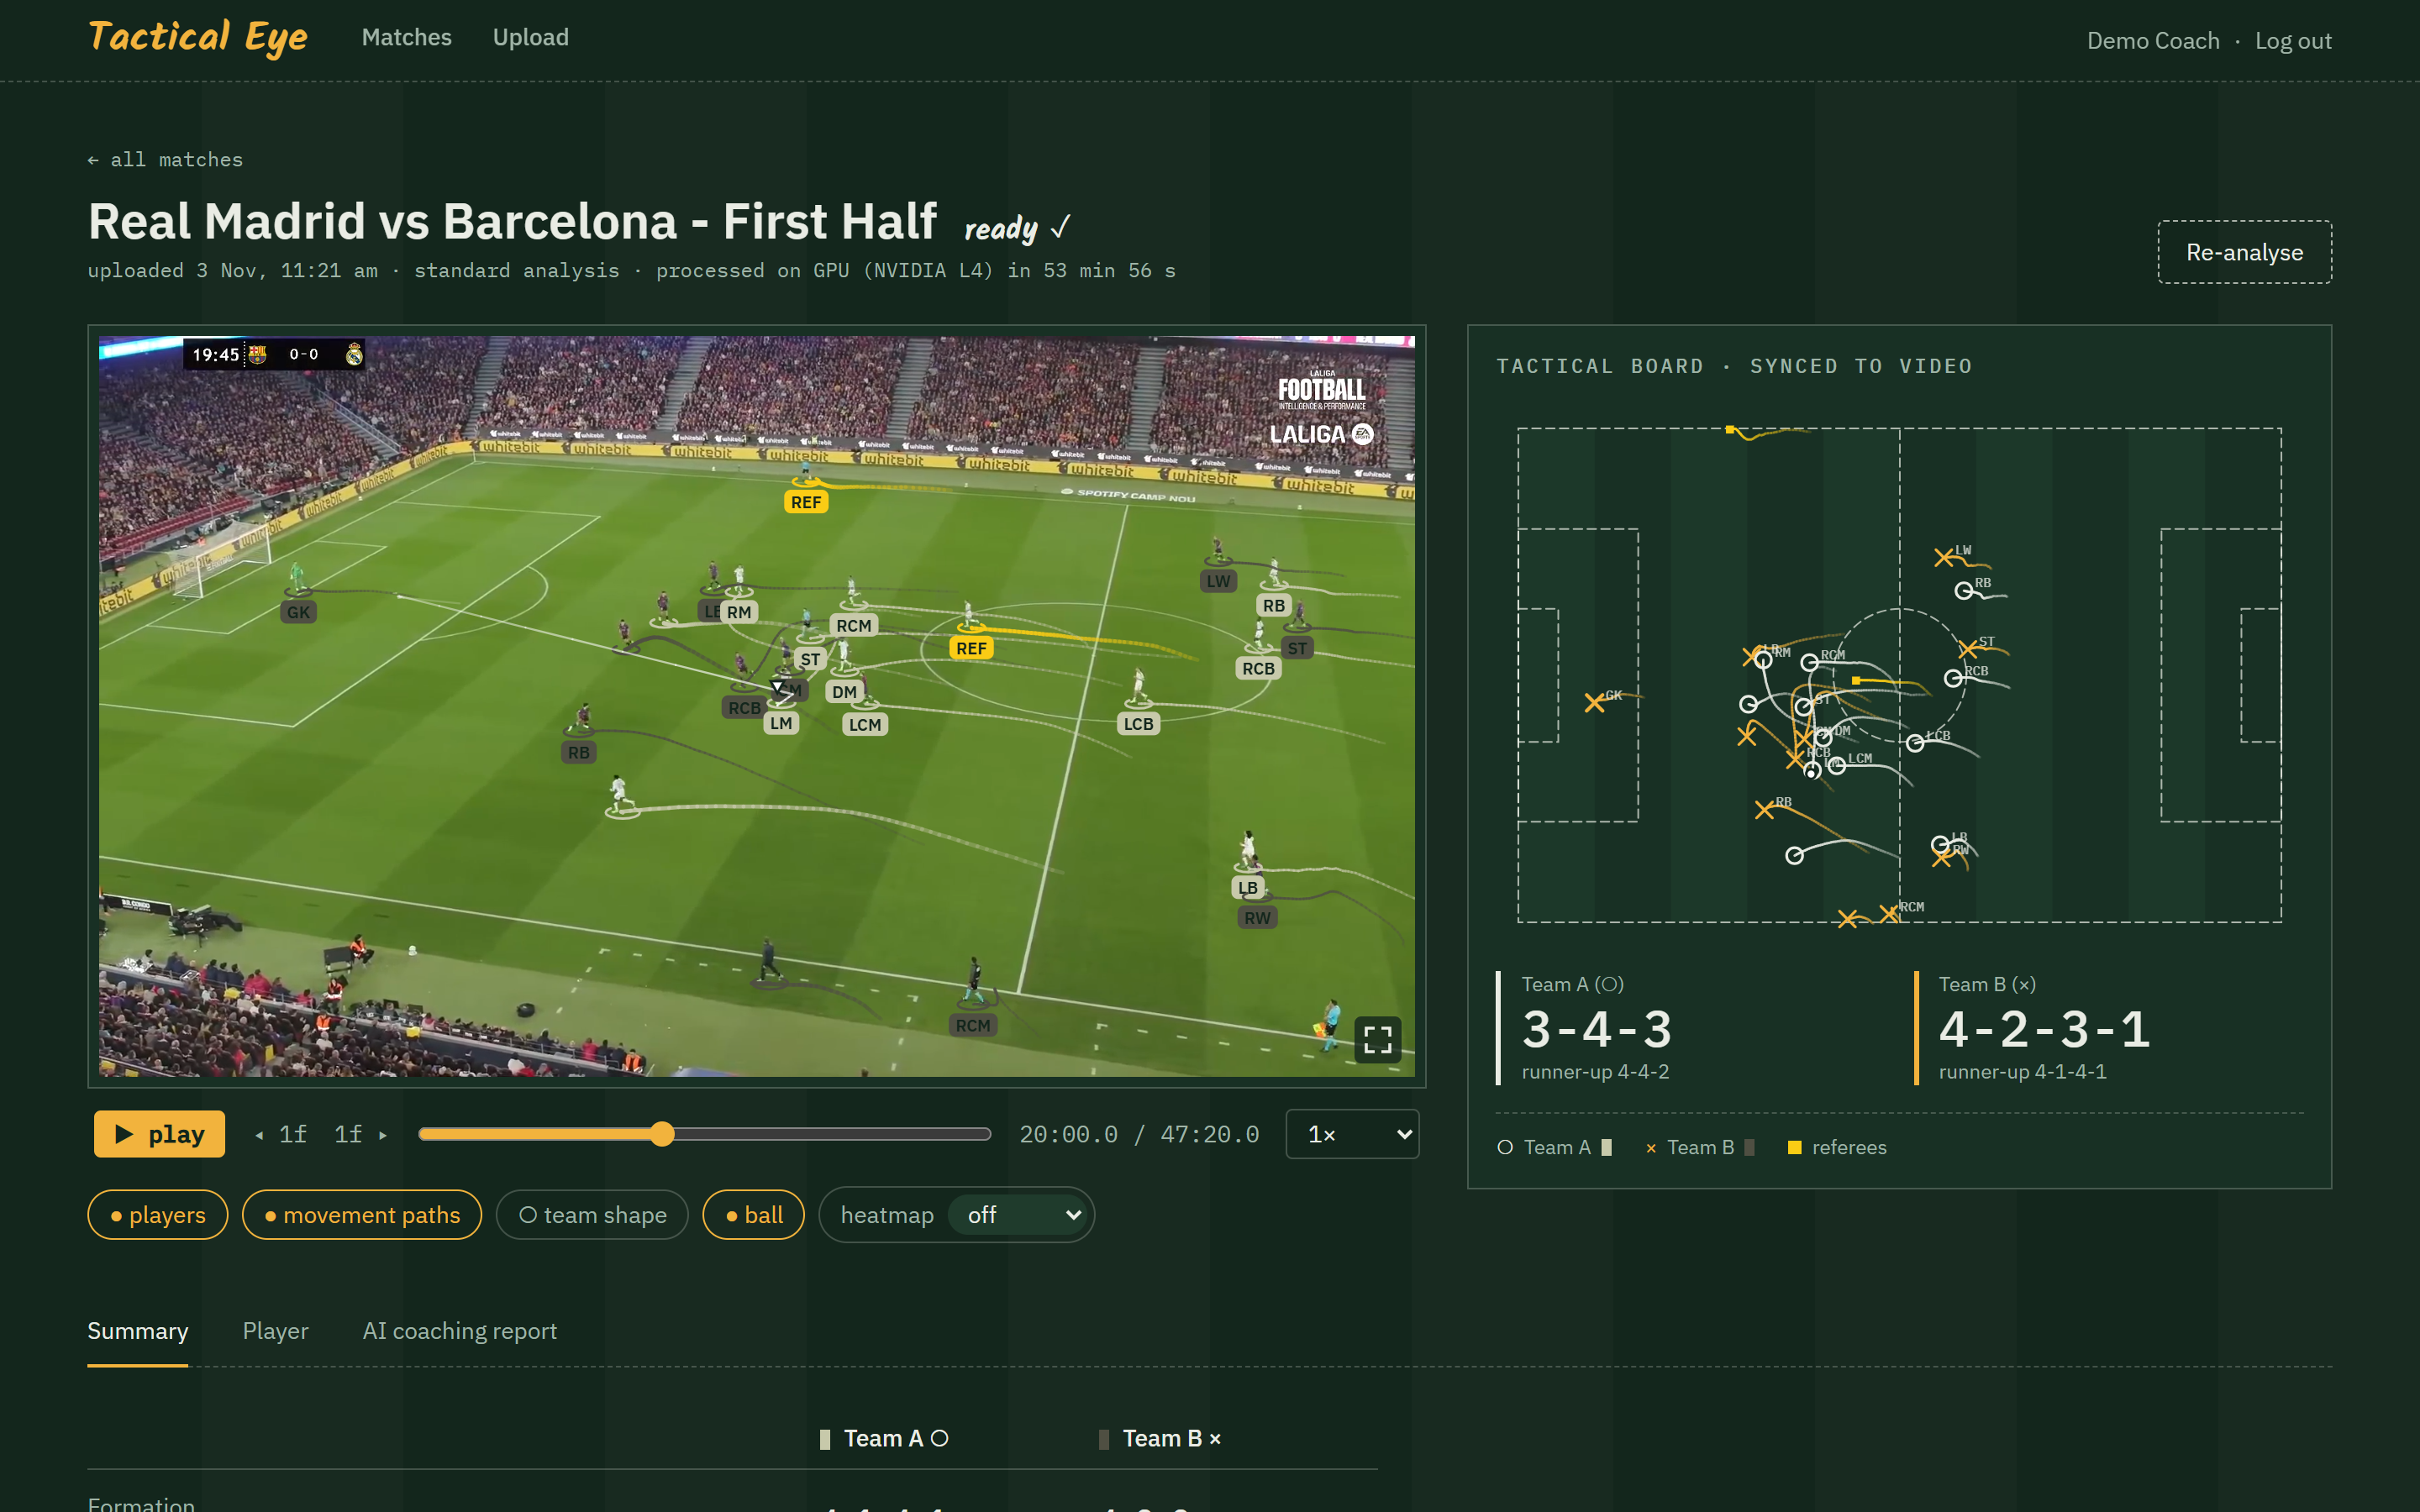
\includegraphics[width=\textwidth]{11_match_page}
	\caption{The analysis page of a full half: video overlays, tactical board and the formations of both teams}
	\label{fig:intro-analysis}
\end{figure}

The platform is a distributed system of four services. A React dashboard runs in the browser; a Node.js API handles accounts and uploads and puts analysis jobs on a Redis queue; a Python AI worker takes the jobs and runs the computer vision pipeline, optionally on a rented cloud GPU; and the API can ask a language model on Azure OpenAI to write the report. Every service runs in a Docker container, and a CI/CD pipeline tests the code and publishes the images.

The platform works from a single broadcast camera, so it only sees what the camera shows. It measures positions, movement and shape, not events such as passes or shots, and because players keep leaving the picture it labels them by position (left back, striker\dots) instead of by name. I tested it on five 30-second Bundesliga clips~\cite{dfl} and on two full halves of about 48 minutes each.

\section{Structure of the thesis}

\autoref{ch:user} is the user documentation: what the software is for, what it needs, how to install it, and every function of the dashboard with its messages. \autoref{ch:developer} is the developer documentation: requirements, architecture, data design, the analysis pipeline, the modules and the main implementation decisions. \autoref{ch:testing} describes the automated tests, the accuracy check against hand-annotated frames and the runs on full halves. \autoref{ch:conclusion} closes with what I learnt.
